 

\documentclass[conference]{IEEEtran}

\usepackage[nolist]{acronym}
\usepackage[backend=bibtex]{biblatex}
\usepackage{graphicx}
\addbibresource{sdn.bib}
% correct bad hyphenation here
\hyphenation{op-tical net-works semi-conduc-tor}

\begin{document}
	%
	% paper title
	% can use linebreaks \\ within to get better formatting as desired
	\title{Comparing caching approaches with \ac{sdn} for \ac{iot} applications}


	% author names and affiliations
	% use a multiple column layout for up to three different
	% affiliations
	\author{\IEEEauthorblockN{Florian Weidner}
		\IEEEauthorblockA{Philipps-University Marburg, Germany\\
			Department of Mathematics and Computer Science, Distributed Systems Group\\
			February 09, 2024\\
	}}

	% make the title area
	\maketitle

	\begin{abstract}
	%\boldmath
	\ac{iot} applications are generating huge amount of data. To be able to process the data efficiently, new strategies are needed. Caching data at the edge of the network turnd out to lower the energy consumption, reduce the network latency and lower request to the core network in the cloud. \ac{sdn} is a technology that fits to manage the caching strategies and hide the complexity to the users. In this paper we will summerize \ac{sdn} witch it's advantages and challenges, general applications as well as applicaitons in \ac{iot}. We will compare different caching strategies using \ac{sdn} for \ac{iot} applications, showing the development of archtectures over time. The first architecture is a early approach using \ac{sdn} for cooperative caching in \ac{isp} networks, using the priority of the data to make the caching descions. The second architecture also considers the lifetime of data in a transient \ac{iot} network. The third architecture uses the \ac{mfo} algorithm to optimize the caching strategy and clusters the network to get a better \ac{qoe}.
	\end{abstract}

	\begin{IEEEkeywords}
	\ac{sdn}, \ac{iot}, edge caching
	\end{IEEEkeywords}

	\IEEEpeerreviewmaketitle

	\section{Introduction}
	\label{sec:introduction}

	With the development of the internet and the increasing complexity of networks, the management and configuration of them become more complex and time consuming. Technologies like moblie networks, cloud computing, multimedia applications and virtualization have a high need of bandwidth, high accessibility and dynamic network configurations. These requirements are a challenge for traditional networks. 

	Traditional Networks are very hardware-centric. Routers and switches are used to manage the network traffic. The control plane is very tightly coupled with the forwarding by the data plane. Since both are happening on the local device, the configuration and management of the network is very time consuming. \acf{sdn} addresses these issues. It uses a centralized approach for managing the network devices. This leads to easier configuration, more flexible forwarding, enhanced performance and reduced costs. \cite{Jefia2018-pj} \cite{MASOUDI20161}


	In this paper we will first summerize the concept of \ac{sdn} and look at applications, advantages and challanges. In section \ref{sec:sdn-iot} we will focus on the usage of \ac{sdn} in \ac{iot} applications and which problems \ac{sdn} can solve. In section \ref{sec:caching} we deep dive  into edge caching approaches using a \ac{sdn} Controller in \ac{iot} applications. We look at three different architectures showing the development of the edge caching with \ac{sdn}. For each one the architecture is described, the proposed improvemnts explained and the evaluation presented. Finally, we will conclude our findings in section \ref{sec:conclusion}. 

	\section{\ac{sdn}}
	\label{sec:sdn}

	\begin{figure}
		\centering
		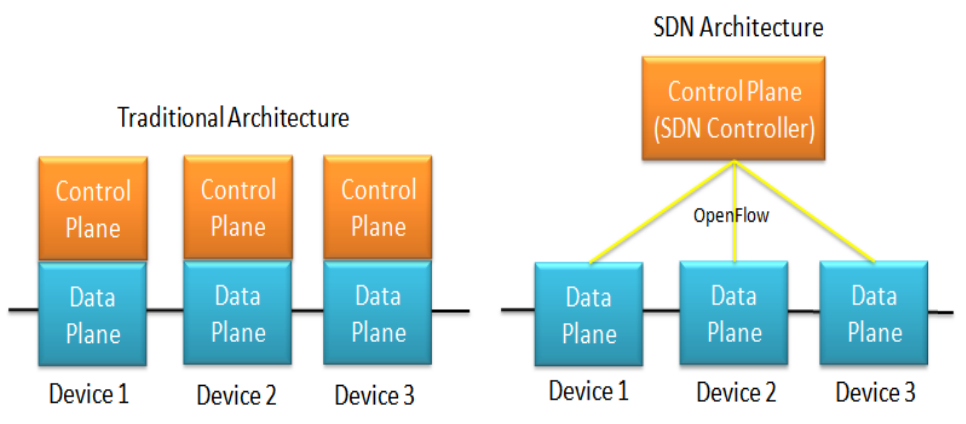
\includegraphics[width=0.5\textwidth]{figures/architecture-compare.png}
		\caption{Traditional Architecture and \ac{sdn} Architecture \cite{Jefia2018-pj}}
		\label{fig:architecture-compare}
	\end{figure}

	\begin{figure}
		\centering
		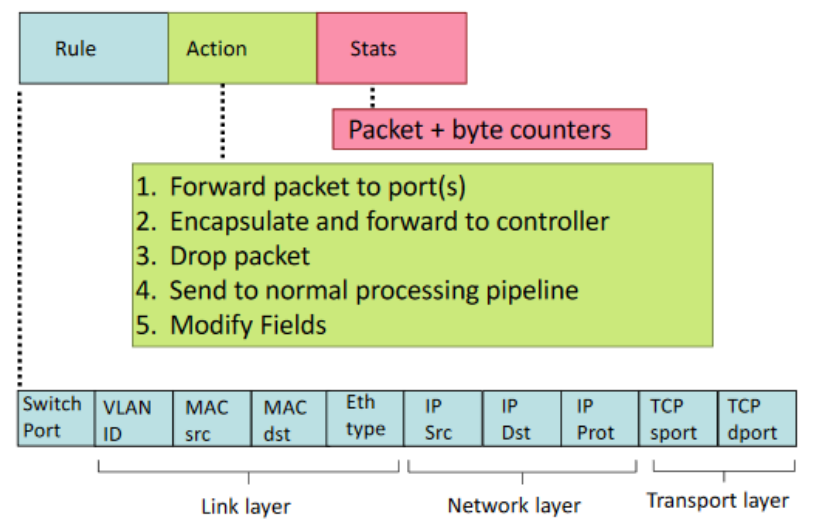
\includegraphics[width=0.5\textwidth]{figures/flow-table.png}
		\caption{Flow Table Entry Representation \cite{nunez2023briefoverviewsoftwaredefinednetworking}}
		\label{fig:flow-table}
	\end{figure}

	\begin{quote}
		"\acf{sdn} is an emerging network architecture
		where network control is decoupled from forwarding and is directly programmable" \cite{sdn-onf} 
	\end{quote}

	This definition is by the \ac{onf} from 2012. \acf{sdn} decouples the control form the data plane. It uses a centralized controller, which has a global view to the network to manage the control plane. The controller can manage and adjust the network and the forwarding configuration of the network devices. There exist different implementations of \ac{sdn} controllers. In \ref{fig:architecture-compare} you can see the difference in the architectures of traditional networks and \ac{sdn} networks. In the traditional architecture, each device has its own control plane to manage the device. In \ac{sdn} the control plane is centralized using the \ac{sdn} controller.

	The main responsitblity of the data plane is forwarding the network traffic. For that, it uses flow tables to determin the forwarding desitnation, which are more complex forwarding tables of traditional routers or switches. More complex decisions based on the information of incoming packtes are possible. In \ref{fig:flow-table} you can se the representation of a flow table entry. An Entry contians three columns. The first one contains the rules to match the incoming packages. The rules can be applied to any part of the datagram. The second one are the actions, that should be executed if the rule matches. The third column is used to store performance metrics on their corresponding rule and action field. \cite{nunez2023briefoverviewsoftwaredefinednetworking}
	The dataplane can also be used, to enable various functions like network inspection, anomaly detection or traffic engineering. \cite{MASOUDI20161} 
	The third plane is the application plane. On that plane software is used to manage the network over the \ac{sdn} controller. There complex funtions can be performed to configure or automate the network trafic, based on the customer needs. \acp{api} are used to comunicate with the hardware in the network.

	The three planes use dedicated interfaces to comunicate. The southbound interface is used to comunicate between the control plane and the data plane. The northbound interface is used to comunicate between the control plane and the application plane. The OpenFlow Protocol, maintained by the \ac{onf} is a commonly used open-source protocol defining an interface for the southbound communication between the controller and the network devices. It defines guidelines and uses \ac{tcp} to update the flow table entires from the control plane. 
	If the controller is distributed the east-westbound \acp{api} can be used to comunicate between the controllers. \cite{nunez2023briefoverviewsoftwaredefinednetworking}


	\subsection{Advantages and Challenges of \ac{sdn}}

	\acf{sdn} has compared to traditional networking several advantages. Here the some of them are summerized.\ac{sdn} provides a better and easier management of the network. All network devices can be controlled from a single point. Also newlly added devices can be easily integrated into the network. \cite{Jefia2018-pj}
	Also the performance of the network will be imporved. It is possible to orchistrate the network traffic centrally. This leads to a better dynamic utilization of the network resources. This also leads to reduced costs. The management of the network is more efficient by using a central software, since there is less need to acces the individual network devices directly. \cite{Jefia2018-pj}
	The forwarding network devices can be simplified. They only need to be able to forward the network traffic and have basic functions to be able to execute the instructions of the contorller, which takes over the management logic. \cite{Hussain2022-tc} With \ac{sdn} the network gets programmable with applicaitons that are installed ot the control plane. The control plane can be dircetly programmed, since it is seperated from the data plane. That also makes automation possible. \cite{Hussain2022-tc}

	But \ac{sdn} also faces some challenges. Research into \ac{sdn} mainly focused on the control plane. The programability of the dataplane is not as advanced as the control plane. With OpenFlow, there is no solution provided for data plane customization. \cite{MASOUDI20161}
	For forwarding devices have a tradoff in flexibilty and performance. General purpose processors provide the highest flexibilty wheras specific standard products are specialized for high performance but lower flexibilty. \cite{Jefia2018-pj}New \ac{sdn} switches are using hardware combinations to achive a better balance between flexibilty and performance.  \cite{MASOUDI20161}
	\ac{sdn} networks are dependent on OpenFlow compatible switches, which limits the scalability. Also the controller needs to be distributed to achive further scalabiltiy, over the limits of a single controller. Splitting the controller leads to typical distributed system problems like latency, fault tolerance, consistency and load balancing. On the other and it also leads to more resilicance, performance and availability. \cite{MASOUDI20161} 
	Since \ac{sdn} is widely being adopted and used, security is getting very important. Controllers are a central target for security threads. With unauthorized access to the controller, the whole network can be compromised. Authentication between controllers and their network devices with \ac{tls} lighten these threads. To achive a secure network protection, an effective security model is mandatory. \cite{Jefia2018-pj}


	\subsection{Applications of SDN}

	SDN networks are used for data centers, enterprise networks, optical networks and even homes and small businesses. \ac{sdn} enables customization and deployment of new services or policies, because of the independence of the control and the data plane. Therefore \ac{sdn} can be used in various network environments. Data centers operate large-scale networks with high traffic, traffic management and many policies. Here \ac{sdn} can be used to manage the network traffic and to provide a better utilization of the network resources. Generally, the same works for enterprise networks. Also for optical networks, the \ac{onf} provides specialized protocols to integrate multiple network technologies. And even for small networks it turns out that using \ac{sdn} is useful. Having a single point of control makes it easier to manage the network. \cite{Jefia2018-pj} 



	\section{Using \ac{sdn} in \ac{iot} Applications}
	\label{sec:sdn-iot}

	\acf{iot} connects devices with limited resources to create various services. \ac{iot} applications are created to mostly collect data and execute tasks for multiple domains, like industrial process systems, traffic monitoring and a large variety  of end-user applications. Often they result in large-scale networks with many heterogeneous devices and protocols. \cite{Li2020-lx} \citeauthor{Li2020-lx} identified that \ac{iot} faces the following problems: 

	\begin{itemize}
		\item Difficulties in control and management, due to the geographically distributed heterogeneous devices in various domains.
		\item Difficult to program and configure, due to different devices with different capabilities, like memory constraints, bandwidth and energy usage.
		\item Long service provisioning, due to the need for a full development cycle, including installing, configuring and testing the devices. 
		\item Resources are not fully used. Devices haven't been completely considered as network resources. \cite{Sahrish2017}
	\end{itemize}

	Missing flexibility, intelligence and application-specific controls, lead to these problems. \ac{sdn} brings a global view on the network and provides capabilities to use network resources efficiently. It reduces the management and brings flexibility to mitigate the problems of \ac{iot}.

	\ac{iot} devices need to be managed a lot, due to the need for configurations, reconfigurations, resource allocations and communication between the devices. \cite{Sahrish2017} The concept of a central controller of a \ac{sdn} network fits the need for central management for all devices in an \ac{iot} network. The controller can be used to activate and deactivate sensors, based on the current needs. Also, the routing of sensor data can be optimized. \cite{Li2020-lx} There exist multiple frameworks for managing \ac{iot} devices with \ac{sdn}. \cite{Sahrish2017} The integration is not trivial, since \ac{sdn} mainly focuses on controlling traffic. It lacks the ability to control sensor hardware and \ac{iot} applications. \cite{Li2020-lx}

	Another application of \ac{sdn} for \ac{iot} is for cellular networks. There are multiple proposals for \ac{sdn}-based cellular networks. With policies and a central controller, abstractions in geographical areas, load balancing, packet inspection and packet processing can be achieved. \cite{Sahrish2017}

	The most common device in \ac{iot} are sensors. For sensor networks, there are also proposals for \ac{sdn}-based solutions. One example is the \ac{wsnsdn}. It consists of a \ac{bs} and several sensor nodes in a classical architecture. The \ac{bs} is controlled by the \ac{sdn} controller, managing the routing instead of the sensor nodes. The sensor nodes also contain flow tables like switches in the \ac{sdn} architecture. \cite{Sahrish2017} There also exist architectures using reconfiguration based on customer needs. That enables sharing a single infrastructure for multiple applications. \ac{sof} also propose reprogramming and retasking the sensor nodes with the control plane. \cite{Li2020-lx} Applying \ac{sdn} to low-power Wi-Fi networks, wireless sensor can achieve a lower power consumption because of low control traffic. \cite{Manguri2022-vp}

	\ac{sdn} based \ac{iot} networks are also used for improved security, enabling authentication and authorization of the devices on the controller. With a global view over the network, approvals of connections can be handled securely by the controller. It also helps run distributed firewalls or detect unauthorized malicious devices. \cite{Sahrish2017} It limits the impact caused by security threads for the most devices in the network. The controller on the other hand promotes to a central target for security threads. \cite{Li2020-lx}

	\ac{iot} and \ac{sdn} are both topics, that are widely researched and also used in the industry. The combination of them is still at an earlier stage. There are many proposals for standards, but no practical implementations are available. Yet, there is still a lot of interest proposing solutions for the different applications already mentioned. \cite{Manguri2022-vp} 

	The main challenge to efficiently use \ac{sdn} networks for \ac{iot} applications is to use all network-wide inforamtion and knowledge to manage the network form the control plane. For that data needs to be coordinated efficiently between the devices. Only that way a collective intelligence can be achieved. Edge Computing tries to process data closer to the source rather that centralized in the cloud. It reduces latency and uses the existing ressouces in the network more efficiently. \cite{edge-computing} \citeauthor{Li2020-lx} states different research approachs to use that concept also in \ac{iot} applications using \ac{sdn}. 

	






	\cite{8777339} \cite{Sahrish2017}

	\section{Caching in \ac{iot} with \ac{sdn}}
	\label{sec:caching}

	Next to edge computing, caching data on the edges of the network is another strategy to optimize the usage of network resources, ensuring lower network latency, energy consumption and higher availability. \cite{caching-1} \cite{caching-2} \cite{caching-4} Without caching, popular content will be transmitted repeatedly, wasting network resources. Especially devices receiving the same information simultaneously. Often the content needs to be location-sensitive, displaying different information on different locations of the world and often the cached contents are only used by the devices in the same areas. To demonstrate the effect of caching  for latency and energy consumption we can look at the results of the caching strategy proposed by \cite{caching-1}. In figure \ref{fig:energy-caching} you can see that the total energy consumption decreases with the cache size. With no caching the energy consumption stays the same. If you use caching, for all strategies the energy consumption decreases significantly by increasing the cache size. The same is shown in figure \ref{fig:latency-caching} for the average response latency. The constant latency with no caching is reduced by caching by more than half.

	The network of a \ac{iot} application using \ac{sdn} and caching at the edge typicaly consists of the following components:
	\begin{itemize}
		\item Edge \ac{sdn} nodes: equiped with caching capabilities in order to serve multiple requests within the domian, without contacting the remote cloud \cite{caching-1} \cite{caching-2}  
		\item \ac{sdn} Controller: The central controller has the possibility to see all edge \ac{sdn} nodes to manage their flow tables. It instructs the edge nodes to perform the caching actions. \cite{caching-1} \cite{caching-2}  
		\item \ac{iot} gateway: used to transmit data between data plane devices, provides authentication and authorization and ensures safety and security. \cite{caching-1}
	\end{itemize}

	Also, due to the huge amount of data collected in \ac{iot} networks, caching is needed to process the data locally, before sending it to the cloud. Otherwise useless data may get sent and stored centrally and unnecessary network traffic is produced. \cite{caching-1} It also challanges the core network to allocate network resources for multiple data requests and replies from consumers. \cite{caching-2}
	A lot of different features are important for caching decisions:

	\begin{itemize}
		\item redundancy and data unavailability when the device is not available. \cite{caching-1}
		\item storage costs
		\item retreival latency
		\item popularity of the data, which is the number of requests for the same data over a certain amount of time. \cite{caching-2}
		\item the lifetime of the data, which is the time the data is valid. \cite{caching-2}
	\end{itemize}

	The caching policies needs to be dynamic. \cite{caching-5} found out that \ac{iot} data follows the Zipf's law with a skewness parameter that can change on a regular basis. The requested data from users of the \ac{iot} applicaion is related to the needs of the users, which is changing during the day. \citeauthor{caching-5} demonstrate that a period of 60 minutes is enough to capture a change in variation in the popularity.  

	The main goal of caching data at the edge is to improve the user experience. Users should not be aware of the complexity of the network. Caching decisions at the edge of a network are complicated, especially with heterogeneous devices. Here \ac{sdn} can help to overcome these challanges with a centralized orchestration. A \ac{sdn} controller can set policies for caching and hide the complexity of the heterogeneous network from the end users. Caching decisions will be decided based on the network-wide information of the controller like the network topology or storage capabilities. When a user makes a request for content produced by some sensor device nearby, the \ac{sdn} controller can identify the location of the content cached and foreward the request to the device, caching the requested data. If the data isn't cached anywhere, the request will be sent to the cloud. \cite{caching-1}
	There are multiple applications where caching at edge nodes can be applied to improve the efficiency of the network:
	\begin{itemize}
		\item Smart health-care: Increased efficiency for processing in real-time with cached data
		\item Smart cities: Large amounts of data are genereated, which must be processed nearby
		\item Internet of vehicles: For vehicle-to-vehicle communication, the collected data is only useful for other vehicles nearby.
		\item Intensive computation systems: Require low latency times.
		\item Wireless sensor networks \cite{caching-1}
	\end{itemize}

	Already existing caching strategies that are designed for traditiondal internet and multimedia contents cannot be directly applied to \ac{iot} applications. Data like Youtube videos or movies won't change over time once available. They can be accessed even years after they are stored. Data stored in \ac{iot} networks are mostly transient, they expire after a certain amount of time. For example timeseries data, like pulse rates or indicators of pollution, the lifetime of data states how long the data is reliable after being generated. After the expiration, the producer uploads it to the cloud. The heterogenity of the edge devices also makes it hard to use already existing caching strategies. \cite{caching-2}

	The following chapters will present different approaches for caching data in \ac{iot} networks with \ac{sdn} at the edge.

	\subsection{Early approach using \ac{sdn} for cooperative caching in \ac{isp} networks}
	\label{sec:priority-caching}
	\begin{figure}
		\centering
		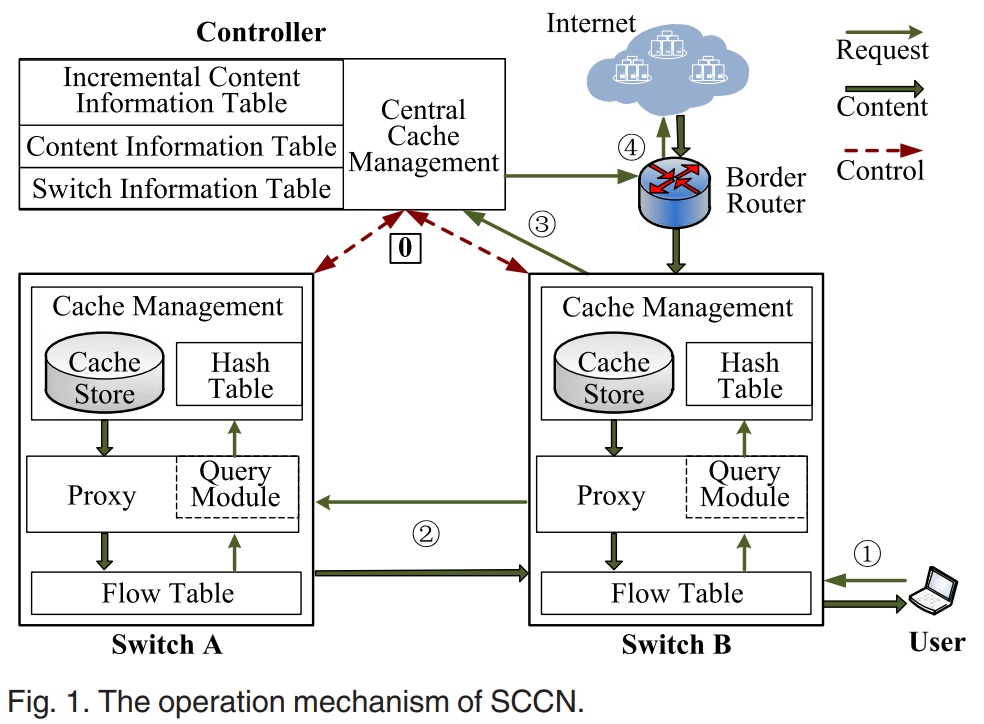
\includegraphics[width=0.5\textwidth]{figures/sccn-architecture.png}
		\caption{The operation mechanism of SCCN \cite{caching-7}}
		\label{fig:sccn-architecture}
	\end{figure}

	In \citeyear{caching-7} \cite{caching-7} proposes \ac{sccn} for \ac{isp} networks using a \ac{sdn} Controller. They propose a \ac{ra} based on a relaxation-rounding technique \cite{ra} to solve the caching problem. They also provide a \ac{ha} based on the concept of Circular Convex Set \cite{heuristcs} to provide a efficient solution usable for practical large scale systems. The \ac{sccn} is implemented with Open vSwitch and Ryu controller.

	\begin{quote}
		"[The] SCCN Controller can detect the most popular contents at the global level, perform intensive computations of content placement decisions and populate new request forward directions to SCCN Switches quickly" \cite{caching-7}
	\end{quote}

	You can see the proposed architecture in figure \ref{fig:sccn-architecture}. The Controller stores three tables of collected data from the network. The \ac{sit} stores information about the switches containing cache capacity and bandwidth. The \ac{cit} tracks cached contents and calculated request counts and the \ac{icit} stores information about recently requestet data that wasn't cached yet. The Controller makes periodic content placement descions based on the information in these tables. When the requested frequency  of a content exceeds a threshold within a time period, an additional caching descion is triggered. 
	If a request is received by a edge node and the data isn't stored, it is forewarded to the Controller, which fetches the data and updates the flow table for future routing. The evaluation of \ac{sccn} compares the \ac{ra} and \ac{ha} algorithm with two algorithms proposed in \cite{caching-8}. The \ac{lg}  has a full replication strategy and caches the K most popular contents for itself. \ac{lgg} doesn't use a replication strategy and only stores a single copy of each content in the network.
	In figure \ref{fig:sccn-result} you can see the results of the evaluation with different cache sizes. You can see that the acceleration ratio (ratio between the saved transmission delay and the original internet delay) and traffic ratio (the ratio between the saved traffic and desired traffic). The \ac{ra} and \ac{ha} algorithm outperform the \ac{lg} and \ac{lgg} algorithm in the acceleration ration over all cache sizes. The \ac{ra} and \ac{ha} have very similar results, showing that the \ac{ha} algorithm is a good approximation for the \ac{ra} algorithm and shoud be used in large scale systems. The \ac{ra} and \ac{ha} algorithm has a similar traffic ratio than the \ac{lgg}, all outperforming the \ac{lg}. The evaluation also states, that the average internet delay, impact of request patterns and large problem sizes don't really affect the better performance of \ac{sccn}.

	\begin{figure}
		\centering
		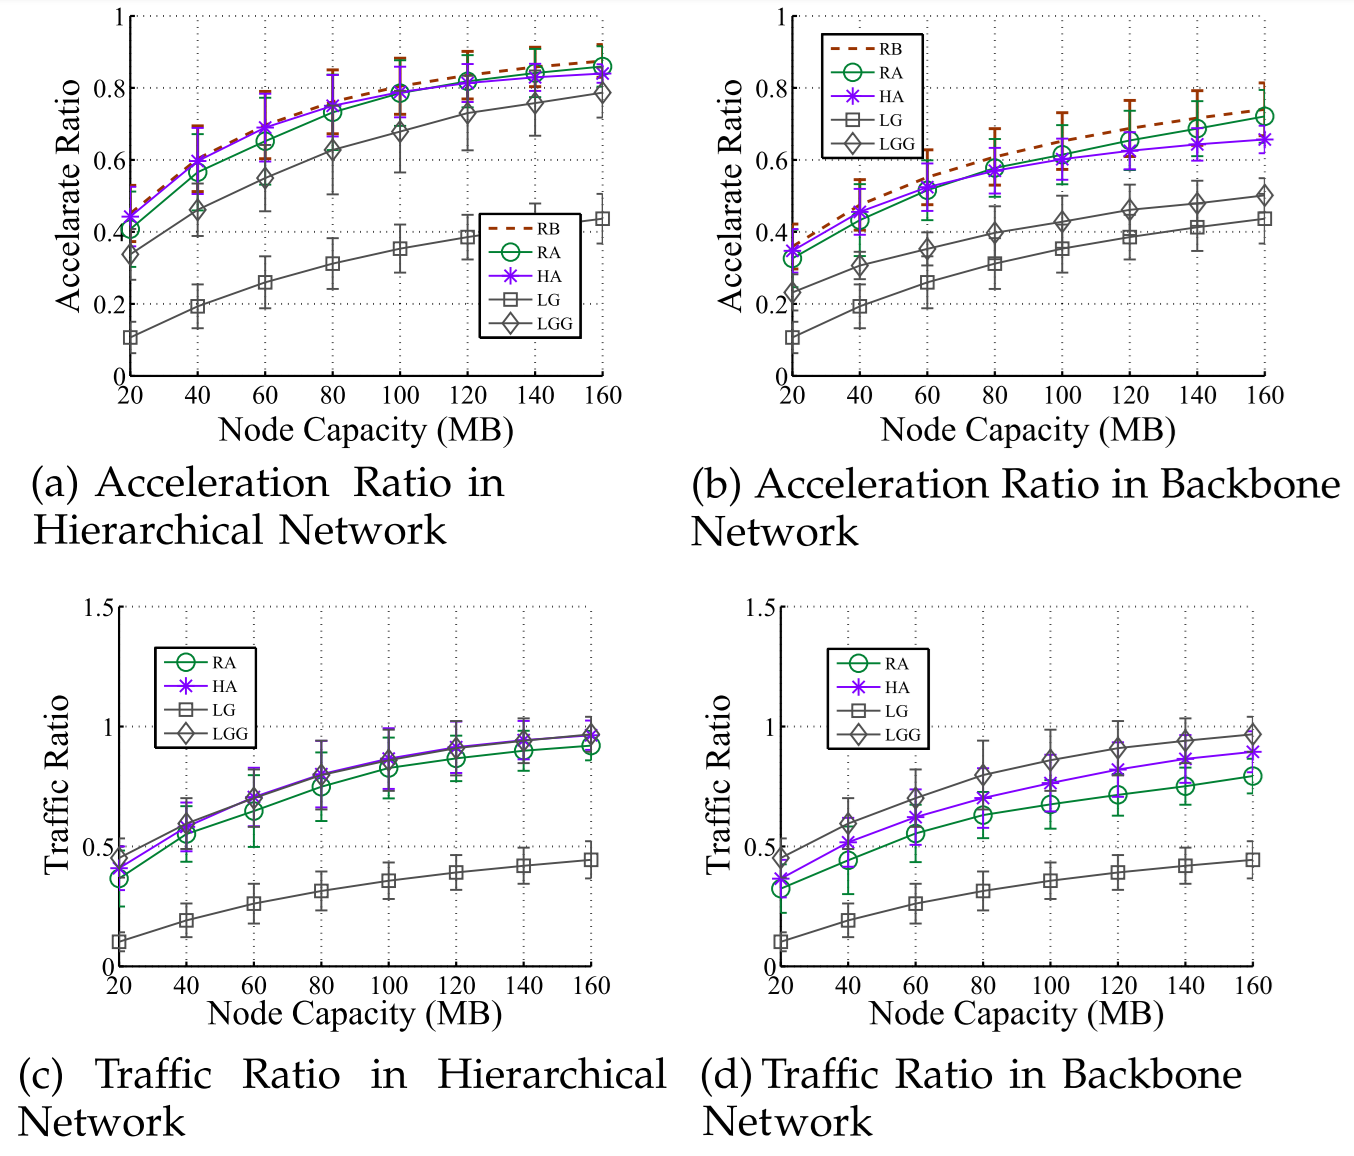
\includegraphics[width=0.5\textwidth]{figures/sccn-result.png}
		\caption{Acceleration ratio and traffic ratio with different cache size \cite{caching-7}}
		\label{fig:sccn-result}
	\end{figure}


	\subsection{Using the lifetime for a caching decision}
	\label{sec:lifetime-caching}

	In \citeyear{caching-2} \cite{caching-2} proposes a caching policy also using a \ac{sdn}-controller. 
	\begin{quote}
		"Such a policy identifies the \textit{IoT contents} to be cached and \textit{the cachers}, by \textit{jointly} accounting for the \textit{IoT content popularity and lifetime}" \cite{caching-2} 
	\end{quote}

	Their goal was to prioritze the cache hit ratio for the most popular contents which have a longer lifetime expectancy. The policy should reduce the retreival latency and maximaize the content diversity available at the edge domain even more. The policy should run as a network application on top of the \ac{sdn} Controller using the OpenFlow protocol for the southbound interface. They define the optimal content placement through an \ac{ilp} problem, that include their named objectives. They claim to be the first caching optimization aproach in a distributed edge domain, that are taking the popularity and the lifetime of \ac{iot} data into account. The idea is, that caching very popular content with only a very short lifetime left is less usefull than less popular content with a longer lifetime. Over the longer livetime the data may have more total requests that the popular one.
	The \ac{sdn} Controller instructs the caching actions at regular intervals. Due to the change of popularity over time \cite{caching-5} they decided to set the intervall at 60 minutes. The \ac{sdn} nodes are then storing the data unitl the data lifetime expires or a new caching decision is made. The \ac{sdn} controller monitors the topology and measures the packet loss probability and the link delay to estimate the content retreival latency. Using the OpenFlow protocol it also monitors the capabilities and content statistics of the \ac{sdn} nodes. That gives information about the amount of flow table entries or buffer sizes of the switches. Also the request arrival rates is summed up, by giving the Controller information about all content requests. These informations are used to make the caching decisions.
	If a node needs to get certain data, it sends a request to the controller, which injects the forwarding rules into the flow table of the \ac{sdn} node, so that it can retreive the data from the cacher directly. To maximize the content diversity, they store only one content copy in the edge network, similar like the \ac{lgg} algorithm of \cite{caching-8}. That reduces traffic transit costs, because more space is available for distinct data and therefore less traffic has to leave the domain requesing data at the cloud. The ability of the \ac{sdn} Controller to use load balancing helps against intra-domain congestion problems. 
	For the optimal content placement they formulate the problem as an \ac{ilp} problem. It is a NP-hard problem, which makes it computationally intensive and impractical for large-scale applications. Therefore, they propose a heuristic algorithm using a greedy approach to find near-optimal solutions more efficiently. This heuristic evaluates factors such as node storage capacity, network link bandwidth, and the transient nature and popularity of IoT content to make caching decisions.
	The evaluation of their caching policy shows that it outperforms other caching strategies in terms of cache hit ratio, content diversity, and retrieval latency. They tested their solution in three scenarios to the benchmark of \ac{mpc} which is an aproach based on the discussed algorithm of \cite{caching-8} in section \ref{sec:priority-caching}. In all three scenarios \ac{mpfc} achieved lower content retreival latency, higher cache hit rates and higher freshness probabilities.
	In figures \ref{fig:lifetime-latency}, \ref{fig:lifetime-hitrate} and \ref{fig:lifetime-freshness} you can see the results of the first scenario. You can see that the content retrieval latency and the cache hit rate from \ac{mpfc}(black lines) is better on all cache sizes than \ac{mpc}(blue lines). For the freshnes probability, with increasing cache size, the freshness probability of \ac{mpfc} equals to \ac{mpc}. The paper proves that the usage of the content's lifetime is improving the caching descions in \ac{iot} networks.

	\begin{figure}
		\centering
		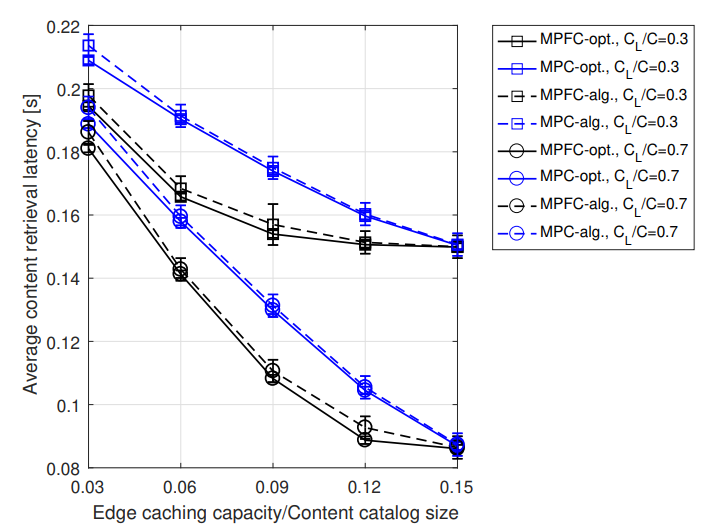
\includegraphics[width=0.5\textwidth]{figures/fresh-latency.png}
		\caption{Average content retrieval latency \cite{caching-2}}
		\label{fig:lifetime-latency}
	\end{figure}
	\begin{figure}
		\centering
		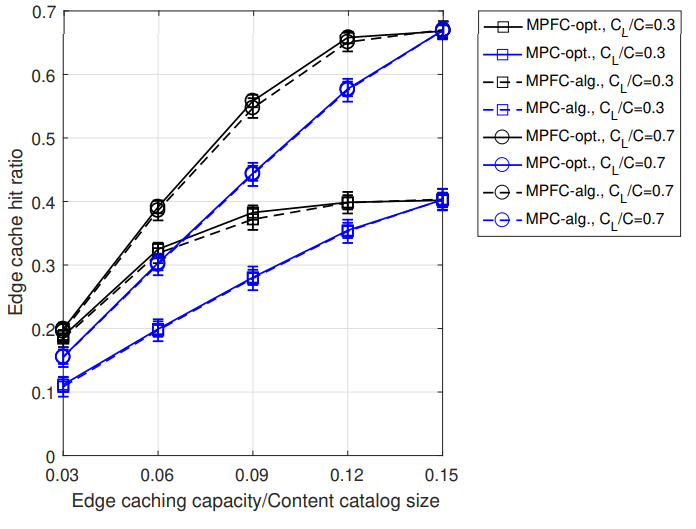
\includegraphics[width=0.5\textwidth]{figures/fresh-hitrate.png}
		\caption{Average content retrieval latency \cite{caching-2}}
		\label{fig:lifetime-hitrate}
	\end{figure}
	\begin{figure}
		\centering
		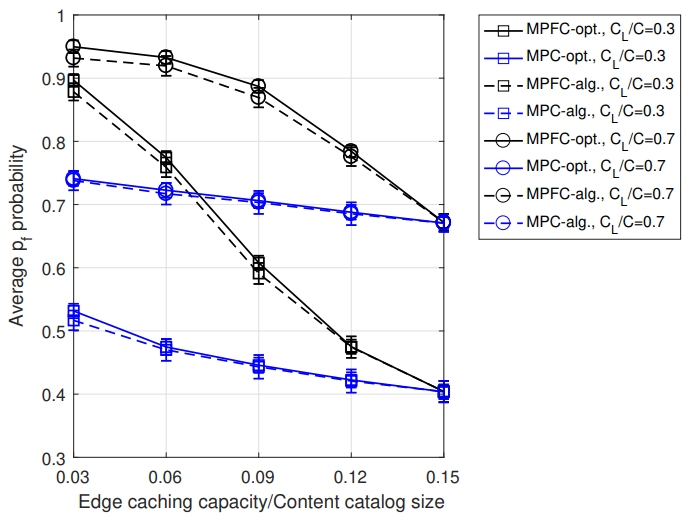
\includegraphics[width=0.5\textwidth]{figures/fresh-freshness.png}
		\caption{Average content retrieval latency \cite{caching-2}}
		\label{fig:lifetime-freshness}
	\end{figure}

	\subsection{Moth-flame optimization algorithm}
	\label{sec:mfo-caching}

	\begin{figure}
x		\centering
		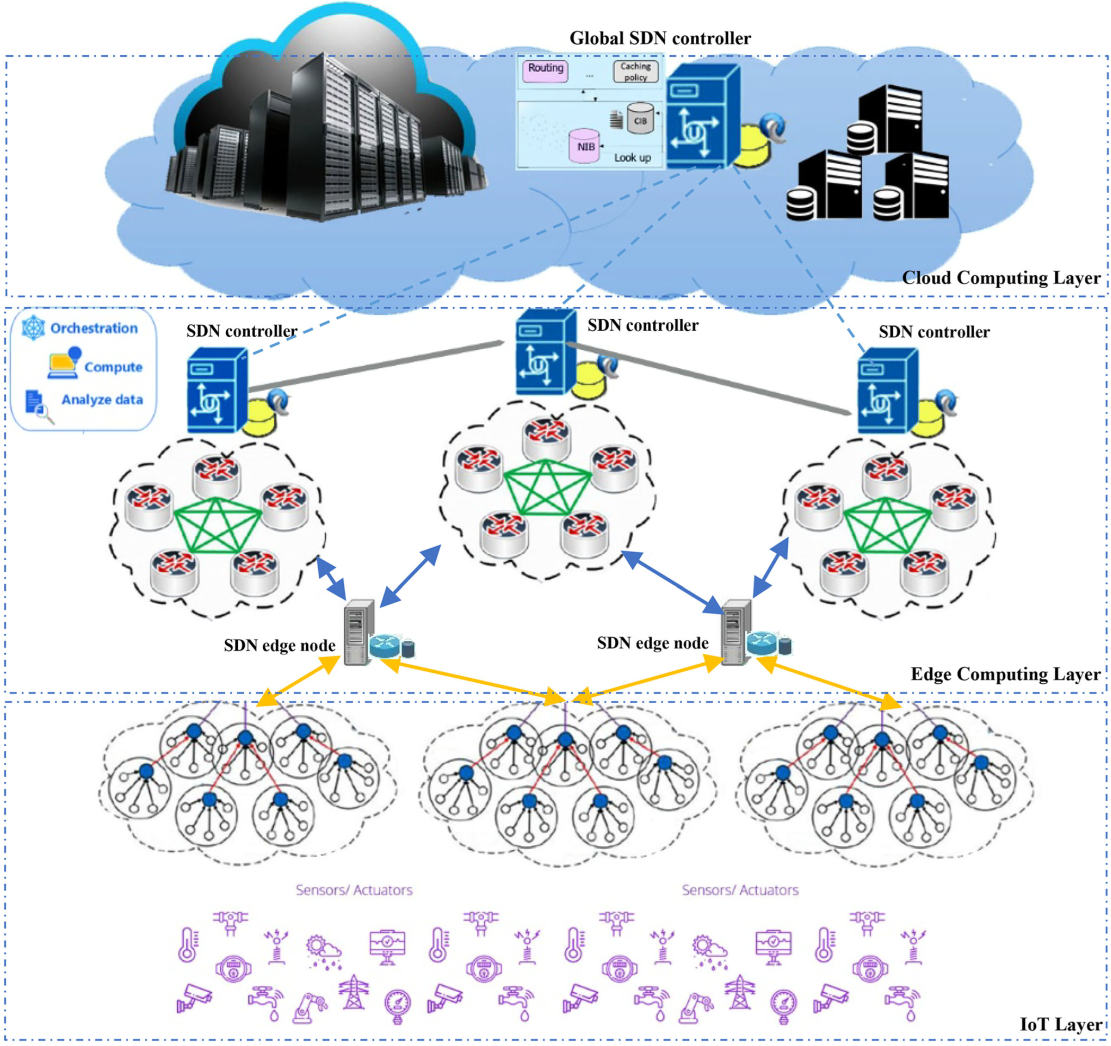
\includegraphics[width=0.5\textwidth]{figures/mfo-architecture.png}
		\caption{The structure of the proposed model \cite{caching-2}}
		\label{fig:lifetime-freshness}
	\end{figure}

	In \cite{caching-1} from \citeyear{caching-1} the authors propose a caching strategy using the \acf{mfo} and cluster the network to get a better \acf{qoe}. It is a population-based metaheuristic inspired by the navigation behavior of moths. Light sources cause moths to fly in a straight line toward them and fly spirally around a light source when very close. They are using the algorithm to group similar content and determine the optimal locations for caching certain data. They cluster the edge nodes and select cluster heads using their propsed algorithm \ac{mfo-chs}.
	In their architecture, also uses \ac{sdn} with a centralized \ac{sdn} Controller. For southbound communication it uses the OpenFlow protocol and for the northbound interface RESTful APIs. For the caching decisions, they use two policies, one for decision-making and one for caching replacement. The first one decides with the \ac{mfo-ec} algorithm on a time intervall what data should be cached where. The replacement policy states which data should be deleted, if the cache, the decision-making policy selected, is full. The \ac{sdn} Controller uses topology information and \ac{iot} data to make caching decisions. The algorithm also uses the content freshness and the content popularity as features to make caching descions. From these two features, a caching weights are calculated, which are then used by the \ac{mfo-ec} algorithm. 
	To create a efficient environment to be able to process massive amounts of data, the authors propose to use \ac{iot} clusters. It further reduces the latency and energy consumption in the network, which leads to better \ac{qoe} for the users. Edge networks are created to be able to better use and share their computational power and resources. With the \ac{sdn} Controller this complexity is hidden to the users. The MFO-CHS algorithm is used to dynamically select the cluster heads. Selecting the best cluster head brings lower end-to-end latency and packet drops. The algorithm tries to select the "fitest" node in the cluster and ensure that the network's energy consumption is at the minimum. For the fitness function, the distance between nodes, the residual energy of the node the priority assigned to the node is taken into account by the \ac{mfo-chs} algorithm. Nodes get priority if they need lower latency or transfer critical data. The clusters are changing over time, adapting to the state of the network. After simulating, the authors found out that their proposed caching strategy outperforms other caching strategies in terms of energy consumption, cache hit rate and average response latency. You can see the results in figures \ref{fig:energy-caching}, \ref{fig:latency-caching} and \ref{fig:latency-caching}. They compare their architecture to different caching strategies. The best architecture the \ac{mfo} architecture is compard to, is a lifetime-based architecture called \ac{lcc} from \cite{caching-6}, which proposes a caching strategy based on the lifetime and popularity of the data, but without using \ac{sdn} like the presented strategy \cite{caching-2} in section \ref{sec:lifetime-caching}. You can see that it outperforms the \ac{lcc} strategy in all three metrics by a bit. The evaluation shows that using the moth-flame algorithm and clustering the network improves the network efficiency.

	\begin{figure}
		\centering
		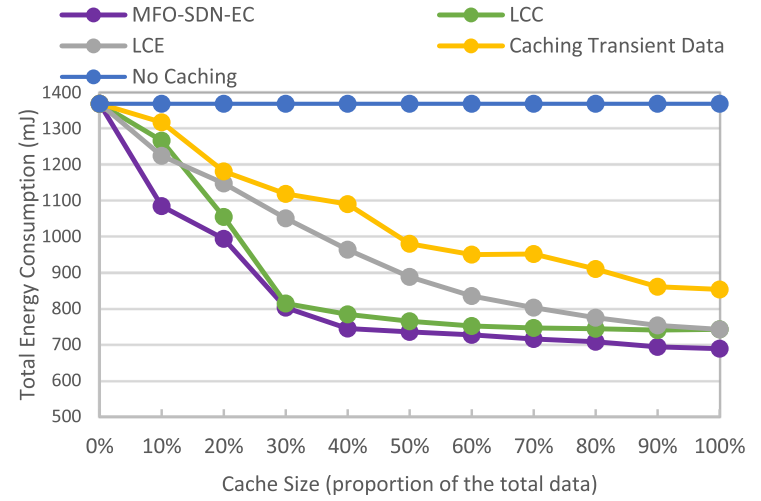
\includegraphics[width=0.5\textwidth]{figures/energy-caching.png}
		\caption{Total Energy Consumption (mJ) VS cache size \cite{caching-1}}
		\label{fig:energy-caching}
	\end{figure}

	\begin{figure}
		\centering
		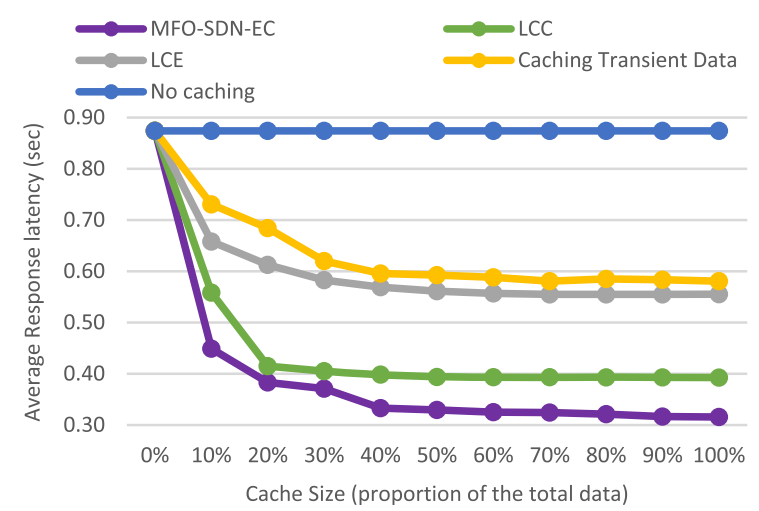
\includegraphics[width=0.5\textwidth]{figures/latency-caching.png}
		\caption{Average Response latency (sec) VS cache size \cite{caching-1}}
		\label{fig:latency-caching}
	\end{figure}

	\begin{figure}
		\centering
		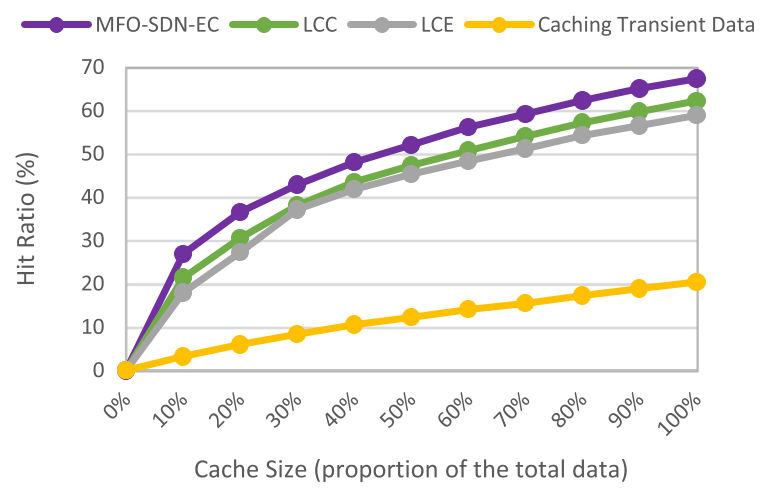
\includegraphics[width=0.5\textwidth]{figures/hitrate-caching.png}
		\caption{Hit Ratio VS cache size \cite{caching-1}}
		\label{fig:latency-caching}
	\end{figure}

	\section{Conclusion}
	\label{sec:conclusion}

	After introducing the topic, we summerized the concept of \ac{sdn} and looked at applications, its adventages and challanges. Then we focused on the usage of \ac{sdn} in \ac{iot} applications and why it helps to overcome problems of \ac{iot} applications on a large scale. We focused on using edge caching managed by a \ac{sdn} controller to improve the network efficiency. We presented three different papers showing the evolution of caching strategies in \ac{iot} networks with \ac{sdn}. The first paper \cite{caching-7} proposed a caching strategy for \ac{isp} networks using the contents priority to make caching descions for the edge nodes. The second paper \cite{caching-2} extended the caching policy by using the priority and the lifetime of the data to make caching decisions. The third paper \cite{caching-1} proposed a caching strategy, taking priority and lifetime of the data into account, using the \ac{mfo} algorithm and clustering the network to improve the efficiency even more.

	\printbibliography
	\begin{acronym}
		\acro{sdn}[SDN]{Software-defined Networking}
		\acro{iot}[IoT]{Internet of Things}
		\acro{onf}[ONF]{Open Networking Foundation}
		\acro{tls}[TLS]{Transport Layer Security}
		\acro{api}[API]{Application Programming Interface}
		\acroplural{api}[APIs]{Application Programming Interfaces}
		\acro{tcp}[TCP]{Transmission Control Protocol}
		\acro{wsnsdn}[WSNSDN]{Software-Defined Wireless Sensor Network Framework }
		\acro{bs}[BS]{Base Station}
		\acro{sof}[SOF]{Sensor OpenFLow}
		\acro{mfo}[MFO]{Moth-Flame Optimization}
		\acro{ilp}[ILP]{Integer Linear Programming}
		\acro{mpc}[MPC]{Most Popular Contents}
		\acro{mpfc}[MPFC]{Most Popular Fresh Contents}
		\acro{mfo-ec}[MFO-EC]{Moth-Flame Optimization-Edge Caching}
		\acro{mfo-chs}[MFO-CHS]{Moth-Flame Optimization-Cluster Head Selection}
		\acro{lcc}[LCC]{Lifetime-based Cooperative Caching}
		\acro{sccn}[SCCN]{SDN-based Cooperative Cache Network}
		\acro{isp}[ISP]{Internet Service Provider}
		\acro{ra}[RA]{Relaxation Algorithm}
		\acro{ha}[HA]{Heuristice Algorithm}
		\acro{lgg}[LGG]{Local-Greedy-Gen Algorithm}
		\acro{lg}[LG]{Local-Greedy Algorithm}
		\acro{sit}[SIT]{Switch Information Table}
		\acro{cit}[CIT]{Content Information Table}
		\acro{icit}[ICIT]{Incremental Content Information Table}
		\acro{qoe}[QoE]{Quality of Experience}
	\end{acronym}

% that's all folks
\end{document}


